\thispagestyle{empty}

\section{Introducere}

\usetikzlibrary{positioning,fit}

Tema acestui proiect este \textbf{„Fuziune Tesla--Meta”}, interpretată ca o fuziune strategică (totală sau parțială) între două organizații cu ADN tehnologic foarte diferit: Tesla (mobilitate electrică, sisteme embedded, fabricație, date de flotă, actualizări OTA) și Meta (platforme sociale, infrastructură cloud/AI, Realitate Virtuală/Augmentată, ecosisteme de conținut și interacțiune).

Fuziunea are la bază o idee simplă, dar cu impact major: \textbf{timpul petrecut în mașină atunci când vehiculul este oprit} (la semafor, în trafic bară la bară, în parcare, în stații de încărcare) poate fi transformat din „timp pierdut” în \textbf{timp util sau recreativ}, printr-o experiență VR/AR sigură, controlată și integrată nativ cu automobilul. În acest scenariu, utilizatorul poate:
\begin{itemize}[leftmargin=1.2cm]
\item participa la ședințe sau sesiuni de colaborare în VR;
\item consuma conținut imersiv (sport, filme, tururi virtuale, jocuri);
\item primi informații contextualizate (status încărcare, ETA, recomandări) fără a interfera cu condusul;
\item folosi „micro-sesiuni” de training/learning în intervale de 2--10 minute.
\end{itemize}

\textbf{Scenariul considerat:} se creează o entitate comună, \textbf{Tesla--Meta Mobility \& Immersive}, cu rol de „unitate de produs” și „platformă tehnologică”, responsabilă să proiecteze și să opereze capabilitățile digitale necesare. În practică, fuziunea poate fi văzută și ca o integrare între anumite departamente cheie, de exemplu:
\begin{itemize}[leftmargin=1.2cm]
\item \textbf{Tesla Vehicle Software \& Platform} (software de bord, OTA, telemetrie, integrare cu hardware-ul mașinii);
\item \textbf{Tesla Data \& Autonomy} (flux de date, siguranță, modele AI, politici de release);
\item \textbf{Meta Reality Labs} (stack VR/AR, interacțiune, device-uri, UX imersiv);
\item \textbf{Meta AI/Infrastructure} (training la scară, streaming, content delivery, MLOps).
\end{itemize}

Deși aceste „divizii” își păstrează instrumentele și practicile istorice, obiectivul fuziunii este crearea unui \textbf{produs comun} și a unei \textbf{platforme comune}. Pentru Tesla, acest lucru înseamnă extinderea automobilului dincolo de „mașină conectată” către un \textbf{spațiu digital}, cu experiențe nativ integrate în sistemul de infotainment și în ecosistemul de servicii. Pentru Meta, înseamnă extinderea VR dincolo de spațiul domestic către un \textbf{context mobil}, cu cerințe de siguranță, conectivitate și latență radical diferite.

Ca rezultat, noua companie își propune să ofere un portofoliu de servicii digitale care, la nivel comercial, seamănă cu un „pachet” de abonamente: experiențe imersive, conținut premium, colaborare și servicii bazate pe AI. În același timp, la nivel operațional, trebuie să garanteze că aceste servicii sunt livrate în condiții de siguranță și conformitate, ceea ce impune o arhitectură care poate demonstra controlul: \textbf{cine} folosește serviciul, \textbf{în ce condiții} poate fi folosit, \textbf{ce date} sunt colectate și \textbf{cum} sunt protejate.

Noua organizație funcționează ca un grup multi-sediu, păstrând centre operaționale și de dezvoltare în locațiile tradiționale (ex.: Austin / Fremont pentru Tesla, Menlo Park pentru Meta), precum și hub-uri de inginerie în Europa (ex.: Berlin) și centre de operațiuni cloud la scară globală. Ca și în scenariile clasice post-fuziune, \textbf{păstrarea identității organizaționale} (echipe, procese, toolchain) vine la pachet cu necesitatea de a crea rapid \textbf{standarde comune} și un \textbf{mod unitar de guvernanță}.

\textbf{Problema:} consiliile de administrație și investitorii celor două companii observă presiuni simultane:
\begin{itemize}[leftmargin=1.2cm]
\item competiție puternică pe experiența digitală (ecosisteme mobile, platforme de conținut, producători auto tradiționali);
\item așteptări crescute ale utilizatorilor pentru servicii „always connected” și personalizare;
\item nevoia de investiții IT semnificative pentru a susține AI, edge computing și conținut imersiv la scară;
\item riscuri ridicate de conformitate (GDPR), securitate și, critic, \textbf{siguranță rutieră}.
\end{itemize}

În acest context, se consideră că doar o entitate comună, mai mare, poate controla costurile de dezvoltare, poate reduce redundanța, poate standardiza platformele și poate livra mai rapid o experiență VR sigură în mașină. Negocierile și validările interne (juridice, de securitate, de compatibilitate tehnică) sunt complexe, iar livrarea valorii trebuie făcută incremental, prin tranziții controlate.

Fuziunea aduce, însă, și \textbf{provocări tipice de integrare}: procese de dezvoltare și release diferite (automotive safety vs. „move fast” în produse digitale), sisteme de identitate separate, modele de date incompatibile, instrumente de observabilitate și management al incidentelor diferite, precum și platforme heterogene pentru streaming/conținut.

În plus, produsul vizat introduce o dimensiune critică, specifică automotive: \textbf{separarea strictă între utilizarea în staționare și utilizarea în mers}. Așadar, chiar dacă experiența țintă este „VR la semafor”, arhitectura trebuie să trateze acest lucru ca un \textbf{control de siguranță} de nivel înalt, nu ca o simplă regulă de interfață. Concret, sistemul trebuie să fie capabil să detecteze în mod robust starea vehiculului (staționar / în mișcare), să blocheze automat experiența VR în momentul în care se detectează inițierea deplasării și să adopte un comportament \textbf{fail-safe} în caz de degradări (senzori indisponibili, conectivitate slabă, erori software).

Această cerință produce efecte în toate straturile arhitecturii: de la business (politici, termeni de utilizare, suport clienți), la aplicații (controlul sesiunii VR, policy enforcement), date (jurnalizare/audit și minimizarea datelor personale), tehnologie (securitate, hardening, observabilitate, management de chei).

Pe baza situației descrise mai sus, strategia inițială a Tesla--Meta Mobility \& Immersive este de a armoniza capabilitățile digitale și infrastructura prin definirea unui \textbf{model unificat de arhitectură de întreprindere}, bazat pe bune practici și standarde relevante, care să asigure: interoperabilitate, securitate, trasabilitate și livrare incrementală.

Pentru a ghida acest program de transformare, conducerea recomandă utilizarea \textbf{TOGAF} (ADM) ca metodă de dezvoltare a arhitecturii, iar \textbf{ArchiMate} ca limbaj de modelare pentru a descrie coerent arhitecturile de business, aplicații, date și tehnologie.

Ca obiectiv de produs, organizația urmărește lansarea pe piață a unui set de capabilități care să permită utilizatorului să folosească VR \textbf{doar când vehiculul este oprit}, cu mecanisme clare de siguranță (detecția stării vehiculului, blocaje de funcționalități în mișcare, monitorizarea atenției) și cu integrare nativă în platforma mașinii.

În acest sens, misiunea de bază este să fie livrată o generație nouă de produse și servicii:
\begin{itemize}[leftmargin=1.2cm]
\item un \textbf{ecosistem de experiențe VR/AR în vehicul} (colaborare, entertainment, training), cu politici de siguranță pentru utilizare exclusiv în staționare;
\item o \textbf{platformă unificată de identitate și servicii digitale} (account, abonamente, plăți, entitlements), valabilă pe device-urile Meta și pe platforma Tesla;
\item un \textbf{lanț de date end-to-end} pentru AI (edge--vehicle, cloud, MLOps) pentru optimizarea siguranței și a experienței utilizatorului;
\item o \textbf{integrare operațională} care reduce redundanța aplicațiilor și crește viteza de lansare a capabilităților.
\end{itemize}

Proiectul urmează \textbf{TOGAF ADM} și folosește diagrame inspirate din \textbf{ArchiMate} pentru a prezenta viziunea, arhitecturile (business, aplicații/date, tehnologie) și planul de migrare.

\subsection{Domeniu de aplicare (scope) și ipoteze}
Obiectivul arhitectural al proiectului este să descrie și să planifice transformarea necesară pentru realizarea produsului „VR în vehicul (în staționare)”, într-o organizație nou creată prin fuziune. Domeniul de aplicare include atât capabilități de business (produse/servicii, operațiuni, suport clienți), cât și capabilități IT (aplicații, date, infrastructură, securitate).

Din perspectiva TOGAF, abordarea urmărește să definească: arhitectura de bază (baseline) rezultată din cele două organizații, arhitectura țintă (target) și una sau mai multe arhitecturi de tranziție (transition). Accentul este pus pe faptul că organizația nu pornește „de la zero”, ci dintr-un peisaj post-fuziune cu soluții existente, costuri istorice și obligații contractuale.

Stakeholderii principali care influențează scope-ul sunt: product management (cerințe și monetizare), inginerie (fezabilitate și performanță), legal/compliance (GDPR, termeni), securitate (zero trust), safety (politici și mecanisme de blocare în mers) și operațiuni (SRE, incident management). Un risc clasic este extinderea necontrolată a domeniului („scope creep”), motiv pentru care scope-ul rămâne centrat pe capabilități direct necesare pentru experiența VR în vehicul.

Acoperim sistemele și procesele relevante pentru:\newline
\textbf{(1)} Identitate și management de cont, \textbf{(2)} servicii digitale în vehicul (runtime, distribuție conținut, UX), \textbf{(3)} date de flotă și AI (telemetrie, feature store, MLOps), \textbf{(4)} monetizare (abonamente, marketplace, drepturi/entitlements), \textbf{(5)} conformitate (GDPR, securitate, politici de siguranță).

În mod explicit, pentru a menține proiectul controlabil, \textbf{nu} intră în scope proiectarea mecanică a vehiculului, optimizarea liniilor de fabricație și nici dezvoltarea completă a hardware-ului headset-urilor VR (se consideră că există produse și road-map-uri dedicate în organizațiile mamă). În schimb, includem punctele de integrare care influențează direct produsul: conectivitate, senzori relevanți pentru starea vehiculului și mecanismele de blocare a funcțiilor în mers.

Ipoteze utilizate:
\begin{itemize}[leftmargin=1.2cm]
\item Fuziunea păstrează brandurile, dar standardizează platformele digitale.
\item Vehiculul este tratat ca \textit{edge node} (compute + senzori + conectivitate).
\item Se urmărește o migrare incrementală cu \textbf{arhitecturi de tranziție}.
\end{itemize}

\subsection{Managementul cerințelor (Requirements Management)}
Într-o fuziune, cerințele se schimbă frecvent: apar constrângeri legale noi, priorități comerciale diferite, dependențe tehnice neprevăzute și riscuri de securitate. De aceea, managementul cerințelor este tratat ca un proces continuu, iar cerințele sunt gestionate pe tot parcursul ADM printr-un backlog controlat, cu trasabilitate către obiectivele de business, către deciziile de arhitectură și către work package-urile din planul de migrare.

Pentru a păstra controlul, cerințele sunt organizate pe niveluri (strategic/tactic/implementare) și sunt validate periodic în ședințe cu Architecture Board. Orice cerință care afectează siguranța (de exemplu „VR doar în staționare”) este tratată ca \textbf{cerință critică} și are asociate: criterii de testare, evidențe de conformitate și mecanisme tehnice de enforcement. În mod similar, cerințele de privacy sunt acompaniate de politici de retenție, clasificare a datelor și justificare (de ce avem nevoie de acel câmp de date).

Un alt element important este armonizarea terminologiei. După fuziune, aceleași concepte pot avea definiții diferite (ex.: „utilizator”, „cont”, „device”, „sesiune”, „consimțământ”). În cadrul managementului cerințelor se definește un vocabular comun și se menține o trasabilitate între termeni și modele de date, pentru a preveni inconsistențe care duc la erori funcționale și la risc legal.

La nivel operațional, backlog-ul este alimentat din:
\begin{itemize}[leftmargin=1.2cm]
\item feedback de la stakeholderi (business, legal, securitate, product);
\item analize de risc (safety, privacy, threat modeling);
\item constrângeri tehnice (latență, conectivitate, compatibilitate vehicul--cloud);
\item lecții învățate din pilotări și lansări incremental.
\end{itemize}

Principalele categorii de cerințe:
\begin{itemize}[leftmargin=1.2cm]
\item \textbf{Cerințe de business}: monetizare prin abonamente, creșterea retenției, reducerea costurilor IT post-fuziune, creșterea vitezei de lansare (time-to-market), satisfacția utilizatorului.
\item \textbf{Cerințe funcționale}: sesiuni VR inițiate și terminate sigur (în staționare), management de conținut, management abonamente/entitlements, profil utilizator, sincronizare multi-device, suport clienți.
\item \textbf{Cerințe de siguranță}: activare VR doar când vehiculul este oprit, detectarea schimbării stării (pornire/mișcare), comportament fail-safe, jurnalizare și audit pentru incidente.
\item \textbf{Cerințe non-funcționale}: securitate (zero trust), confidențialitate (GDPR), disponibilitate, performanță (latență redusă pentru control și streaming), observabilitate (tracing end-to-end), scalabilitate globală.
\item \textbf{Constrângeri}: compatibilitate cu platformele existente, integrare treptată, bugete și echipe, diferențe de procese și toolchain între Tesla și Meta.
\end{itemize}

\textbf{Cerință (rol în proiect):} Se consideră că echipa de arhitectură este coordonată de un \textbf{arhitect principal de întreprindere} în cadrul Tesla--Meta Mobility \& Immersive, care conduce o echipă de arhitecți pe domenii (business, aplicații/date, tehnologie, securitate/safety) și colaborează cu biroul de management al proiectelor și cu managementul operațional.

Organizația are un portofoliu mare de inițiative post-fuziune (integrare identitate, consolidare date, migrare infrastructură, lansare produs VR, conformitate), ceea ce impune o abordare structurată pentru standarde, guvernanță și prioritizare. În acest context, consiliul de arhitectură decide că este necesară o metodă formală (TOGAF) pentru a controla complexitatea, a evita arhitecturi paralele incompatibile și a asigura că fiecare proiect contribuie la arhitectura țintă.

\subsection{Faza Preliminară (TOGAF): pregătirea capabilității de arhitectură}
În faza preliminară stabilim cadrul de guvernanță și modul de lucru pentru arhitectura întreprinderii, astfel încât transformarea post-fuziune să fie controlabilă și repetabilă. Pentru cazul nostru, această fază este critică deoarece produsul țintă atinge simultan domenii cu reguli stricte (safety în automotive, privacy, securitate) și domenii cu ritm rapid (produse digitale, conținut, AI), iar fără un cadru comun există risc mare de fragmentare.

Rezultatul așteptat al fazei preliminare este un set de mecanisme prin care organizația poate:\newline
\textbf{(1)} decide rapid standarde și tehnologii, \textbf{(2)} controla excepțiile, \textbf{(3)} menține trasabilitatea deciziilor, \textbf{(4)} asigura conformitatea proiectelor în derulare cu arhitectura țintă.

În termeni practici, în această fază se stabilește și un \textbf{Architecture Repository} (modele, diagrame, ADR-uri, standarde), precum și un set de \textbf{referințe} pe care echipele le folosesc ca punct de pornire: patterns pentru integrare (API + events), patterns pentru identitate (SSO/MFA/consimțământ), patterns pentru observabilitate (logging/tracing/metrics), precum și un model de guvernanță pentru date (catalog, ownership, acces). Prin această abordare, proiectele paralele din organizație pot evolua în aceeași direcție, fără a crea soluții incompatibile.

\subsubsection{Principii de arhitectură}
\begin{itemize}[leftmargin=1.2cm]
\item \textbf{Platform first}: capabilitățile comune (identitate, date, observabilitate) sunt oferite ca platformă internă.
\item \textbf{Security by design}: control de acces, criptare, audit, model zero trust.
\item \textbf{Privacy by design}: minimizarea datelor personale, separarea PII, consimțământ.
\item \textbf{API-driven integration}: integrare prin API-uri versionate și evenimente.
\item \textbf{Incremental migration}: schimbări mici, reversibile, cu măsurarea beneficiilor.
\end{itemize}

\subsubsection{Guvernanță și roluri}
Se definește un \textbf{Architecture Board} (Enterprise Architect, Security Architect, Data Architect, reprezentanți business) și un proces de aprobare pentru:
\begin{itemize}[leftmargin=1.2cm]
\item standarde și tehnologii aprobate;
\item excepții (waivers) cu termen și plan de remediere;
\item decizii de arhitectură (ADR) și arhiva acestora.
\end{itemize}

\section{Faza A: Viziune arhitecturală}
Faza A (TOGAF ADM) stabilește \textbf{viziunea arhitecturii} și creează un \textbf{context motivațional} pentru provocările de transformare ale organizației Tesla--Meta Mobility \& Immersive. În cazul nostru, viziunea trebuie să răspundă la trei întrebări cheie:
\begin{itemize}[leftmargin=1.2cm]
\item \textbf{De ce?} Pentru a valorifica sinergiile Tesla (vehicul/edge/OTA) și Meta (VR/AI/conținut) și a crea un produs diferențiator: VR în vehicul utilizabil \textbf{exclusiv în staționare}.
\item \textbf{Ce?} O platformă end-to-end (vehicul + cloud + identitate + conținut) care permite sesiuni VR scurte și sigure la semafor/în trafic/în stații de încărcare.
\item \textbf{Cum?} Printr-o transformare incrementală, guvernată, cu principii clare (security/privacy/safety by design) și cu livrabile de arhitectură trasabile către cerințe.
\end{itemize}

Ca parte a fazei A sunt identificate principalele părți interesate (stakeholderi) și preocupările acestora. TOGAF recomandă reprezentarea acestora într-o \textbf{hartă a stakeholderilor}. În plus, pentru fiecare preocupare putem face o evaluare SWOT (puncte tari/slabe, oportunități/amenințări) și putem lega preocupările de obiective inițiale la nivel înalt.

\subsection{Stakeholderi: preocupări și evaluare (SWOT)}
Pentru scenariul „Fuziune Tesla--Meta”, stakeholderii principali sunt:
\begin{itemize}[leftmargin=1.2cm]
\item \textbf{Board (Tesla--Meta)}: profitabilitate, reducerea costurilor post-fuziune, poziționare strategică pe piață.
\item \textbf{Clienți actuali și potențiali}: satisfacție, ușurință în utilizare, stabilitate, încredere și valoare percepută.
\item \textbf{Safety \& Regulatory}: utilizare VR doar în staționare, fail-safe, auditabilitate și responsabilitate.
\item \textbf{Security \& Privacy}: protecția identității și a datelor (GDPR), control acces, criptare, prevenirea abuzurilor.
\item \textbf{Engineering \& Operations}: scalabilitate, observabilitate, costuri operaționale reduse, time-to-market.
\end{itemize}

O evaluare SWOT sintetizată pentru inițiativă:
\begin{itemize}[leftmargin=1.2cm]
\item \textbf{Strengths}: integrare nativă vehicul--cloud, OTA, experiență VR/AI la scară.
\item \textbf{Weaknesses}: diferențe culturale și de guvernanță; sisteme fragmentate post-fuziune.
\item \textbf{Opportunities}: abonamente VR, conținut premium, servicii B2B (training/collaboration).
\item \textbf{Threats}: incidente de safety, breșe de securitate, neconformitate GDPR, reputație.
\end{itemize}

\subsection{Figura 2: Fragment dintr-o vizualizare a părților interesate}
Fragmentul de mai jos identifică doi stakeholderi (Board și Customer) și preocupările lor. \textbf{Satisfacția clienților} este o preocupare comună, iar satisfacția stakeholderilor se rafinează, în final, către \textbf{profit}.

\begin{figure}[H]
\centering
\begin{adjustbox}{max width=\textwidth}
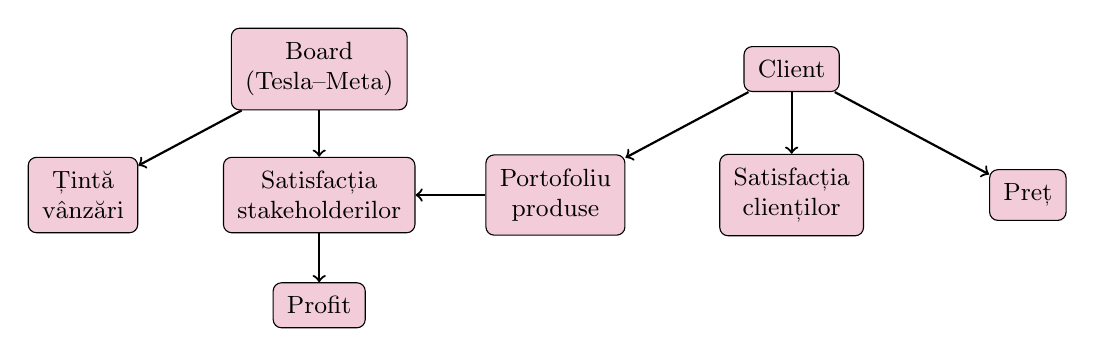
\begin{tikzpicture}[
  x=1cm,
  y=1cm,
  font=\small,
  n/.style={draw, rounded corners=3pt, align=center, inner sep=5pt, fill=purple!20},
  arr/.style={->, thick}
]

% Rândul de jos (ca în exemplul din screenshot)
\node[n] (sales) at (-3,0) {Țintă\\vânzări};
\node[n] (stakeSat) at (0,0) {Satisfacția\\stakeholderilor};
\node[n] (portfolio) at (3,0) {Portofoliu\\produse};
\node[n] (custSat) at (6,0) {Satisfacția\\clienților};
\node[n] (price) at (9,0) {Preț};

% Nodurile de sus/jos
\node[n] (board) at (0,1.6) {Board\\(Tesla--Meta)};
\node[n] (customer) at (6,1.6) {Client};
\node[n] (profit) at (0,-1.4) {Profit};

% Săgeți
\draw[arr] (board) -- (sales);
\draw[arr] (board) -- (stakeSat);
\draw[arr] (stakeSat) -- (profit);

\draw[arr] (customer) -- (portfolio);
\draw[arr] (customer) -- (custSat);
\draw[arr] (customer) -- (price);

% Legătură orizontală (ca în screenshot)
\draw[arr] (portfolio) -- (stakeSat);

\end{tikzpicture}
\end{adjustbox}
\caption{Fragment dintr-o vizualizare a părților interesate (Stakeholder View)}
\end{figure}

\subsection{Motivația: dezvoltarea obiectivelor specifice de business pentru profit}
Driver-ul \textbf{Profit} poate fi rafinat în obiective de business. De exemplu, reducerea costurilor poate fi partiționată în reducerea costurilor de mentenanță și reducerea costurilor de personal, iar creșterea veniturilor poate fi susținută de servicii premium (abonamente VR, conținut, colaborare). Diagrama următoare este o adaptare la tema noastră a structurii din exemplu.

\begin{figure}[H]
\centering
\begin{adjustbox}{max width=\textwidth}
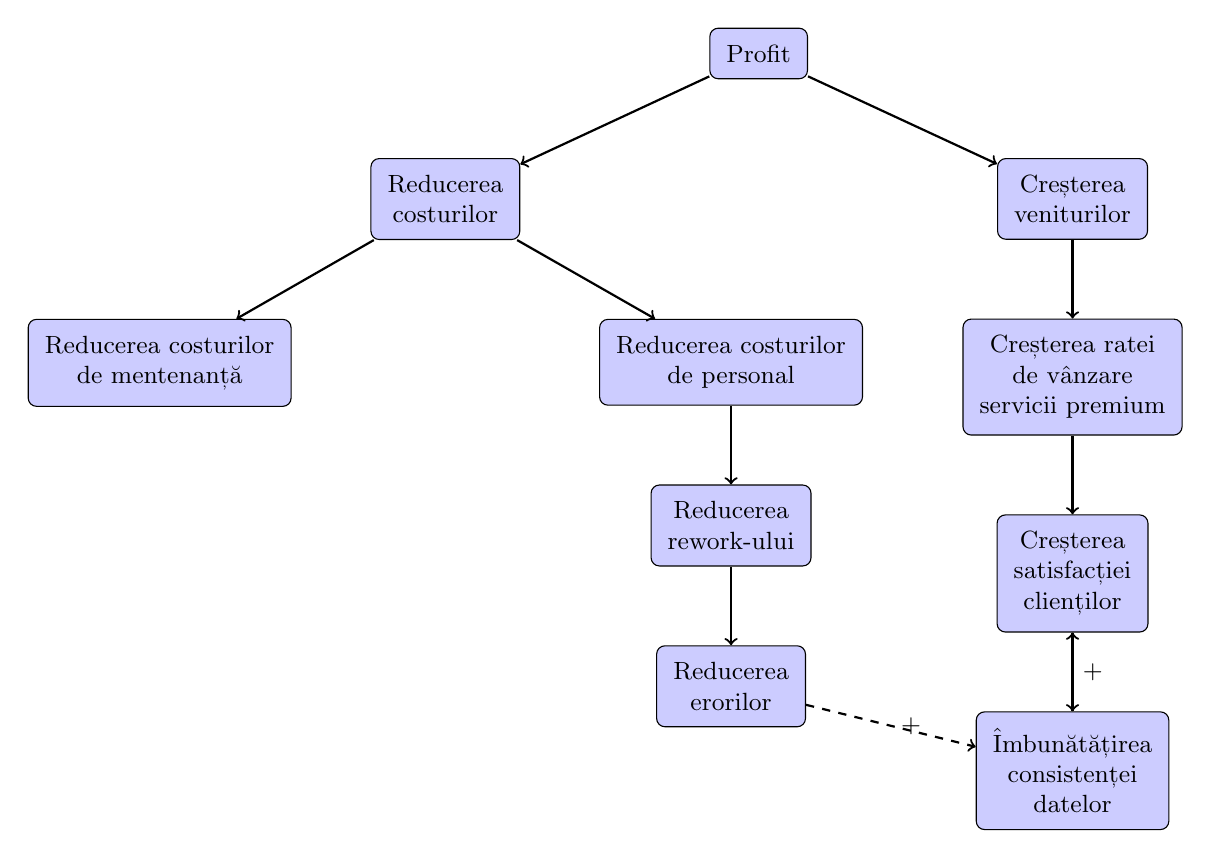
\begin{tikzpicture}[
  font=\small,
  g/.style={draw, rounded corners=3pt, align=center, inner sep=6pt, fill=blue!20},
  arr/.style={->, thick},
  infl/.style={->, thick, dashed}
]

\node[g] (profit) {Profit};
\node[g, below left=10mm and 24mm of profit] (redCosts) {Reducerea\\costurilor};
\node[g, below right=10mm and 24mm of profit] (incRev) {Creșterea\\veniturilor};

\node[g, below left=10mm and 10mm of redCosts] (maint) {Reducerea costurilor\\de mentenanță};
\node[g, below right=10mm and 10mm of redCosts] (personnel) {Reducerea costurilor\\de personal};
\node[g, below=10mm of personnel] (rework) {Reducerea\\rework-ului};
\node[g, below=10mm of rework] (errors) {Reducerea\\erorilor};

\node[g, below=10mm of incRev] (cross) {Creșterea ratei\\de vânzare\\servicii premium};
\node[g, below=10mm of cross] (custSat) {Creșterea\\satisfacției\\clienților};
\node[g, below=10mm of custSat] (dataCons) {Îmbunătățirea\\consistenței\\datelor};

\draw[arr] (profit) -- (redCosts);
\draw[arr] (profit) -- (incRev);
\draw[arr] (redCosts) -- (maint);
\draw[arr] (redCosts) -- (personnel);
\draw[arr] (personnel) -- (rework);
\draw[arr] (rework) -- (errors);
\draw[arr] (incRev) -- (cross);
\draw[arr] (cross) -- (custSat);
\draw[arr] (custSat) -- (dataCons);

\draw[infl] (errors) -- node[right]{+} (dataCons);
\draw[infl] (dataCons) -- node[right]{+} (custSat);

\end{tikzpicture}
\end{adjustbox}
\caption{Figura 3 - Obiective de business asociate driver-ului Profit}
\end{figure}

\subsection{Principii: definiție și modelare}
ArchiMate definește un principiu ca o proprietate normativă a „sistemelor” dintr-un context (inclusiv organizații și unități organizaționale, nu doar IT). Principiile ajută la realizarea obiectivelor de business. TOGAF definește un principiu ca o declarație calitativă de intenție pe care arhitectura trebuie să o îndeplinească; un principiu are o justificare rațională și o măsură de importanță.

Analistul sau proiectantul modelează principiile relevante problemei de proiectare, obiectivele care motivează aceste principii și relațiile dintre ele (influențe pozitive/negative). TOGAF definește un \textbf{catalog de principii} pentru o privire de ansamblu.

\begin{figure}[H]
\centering
\begin{adjustbox}{max width=\textwidth}
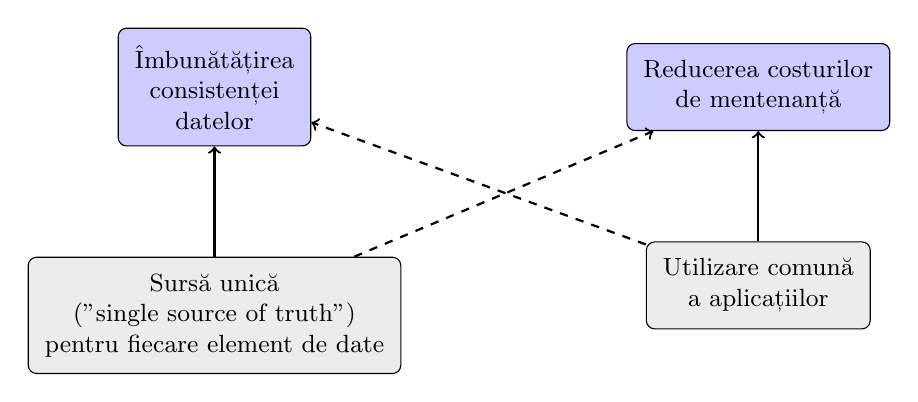
\begin{tikzpicture}[
  font=\small,
  g/.style={draw, rounded corners=3pt, align=center, inner sep=6pt, fill=blue!20},
  p/.style={draw, rounded corners=3pt, align=center, inner sep=6pt, fill=gray!15},
  arr/.style={->, thick},
  infl/.style={->, thick, dashed}
]

\node[g] (dataCons) {Îmbunătățirea\\consistenței\\datelor};
\node[g, right=40mm of dataCons] (maint) {Reducerea costurilor\\de mentenanță};

\node[p, below=14mm of dataCons] (sor) {Sursă unică\\("single source of truth")\\pentru fiecare element de date};
\node[p, below=14mm of maint] (commonApps) {Utilizare comună\\a aplicațiilor};

\draw[arr] (sor) -- (dataCons);
\draw[infl] (sor) -- (maint);
\draw[arr] (commonApps) -- (maint);
\draw[infl] (commonApps) -- (dataCons);

\end{tikzpicture}
\end{adjustbox}
\caption{Figura 4 - Vizualizare a principiilor de business (Business Principles View)}
\end{figure}

\subsection{1. Cum ne asigurăm că Viziunea Arhitecturii răspunde cerințelor părților interesate}
Pentru a ne asigura că viziunea răspunde cerințelor părților interesate:
\begin{itemize}[leftmargin=1.2cm]
\item Identificăm toate părțile interesate implicate, preocupările acestora și factorii culturali post-fuziune.
\item Clasificăm pozițiile și influența, înregistrând rezultatele într-o hartă a stakeholderilor.
\item Ne concentrăm asupra părților interesate cu influență majoră și definim punctele de vedere relevante pentru fiecare.
\item Validăm că preocupările sunt adresate explicit în viziune, prin obiective și principii.
\item Stabilim criterii de acceptanță la nivel înalt și un mecanism de feedback (revizii periodice în Architecture Board).
\end{itemize}

\section{Faza B: Arhitectura afacerii (Business Architecture)}
În faza B (Arhitectura afacerii) din ADM TOGAF, scopul este descrierea modului în care organizația funcționează la nivel de \textbf{structură organizațională}, \textbf{produse/servicii}, \textbf{funcții} și \textbf{procese}. Pentru tema „Fuziune Tesla--Meta”, arhitectura de business este cu atât mai importantă cu cât inițiativa VR în vehicul implică actori diferiți, responsabilități distincte și un lanț de valoare care trece prin zone care, în mod normal, aparțin unor industrii diferite (automotive, software, media/VR, cloud).

După fuziune, Tesla--Meta Mobility \& Immersive este organizată astfel încât să existe o separare clară între activitățile orientate către client și activitățile de execuție/operare, dar și un set de funcții partajate necesare pentru continuitate și conformitate:
\begin{itemize}[leftmargin=1.2cm]
\item \textbf{Front-office partajat (Customer Experience Center)}: suport multi-canal pentru clienți (aplicație mobilă, portal web, call center), onboarding, gestionare abonamente, suport incident VR (sesiuni blocate, incompatibilități, probleme de streaming).
\item \textbf{Back-office Vehicle Operations (Tesla)}: operațiuni legate de vehicul (telemetrie, OTA, validări de siguranță, managementul versiunilor de software din mașină, monitorizare flotă).
\item \textbf{Back-office Immersive Content \& Platform (Meta)}: management de conținut VR/AR, parteneriate, publishing, moderare, recomandări, management de catalog.
\item \textbf{Shared Services Center (SSC) Digital \& Compliance} (funcție partajată): guvernanță și conformitate pentru date (GDPR), procese de audit, managementul consimțământului, politici de retenție, precum și operațiuni de securitate și observabilitate (SRE/SOC).
\item \textbf{Safety Program Office} (funcție transversală): definește politici și controale pentru utilizarea VR \textbf{doar în staționare}, gestionează criterii de acceptanță, testare și evidențe de conformitate.
\end{itemize}

Pentru a asigura continuitatea afacerii și gestionarea perioadelor de vârf (lansări, campanii, update-uri majore), funcțiile partajate includ și capacități de escaladare: personal instruit și proceduri care pot prelua temporar sarcini critice de suport sau triere incidente între echipe.

ArchiMate poate exprima și reprezenta relațiile dintre aceste unități organizaționale, roluri, produse, servicii, funcții și procese. Arhitectura de business oferă astfel contextul pentru arhitecturile de date, aplicații și tehnologie: \textbf{ce} trebuie susținut tehnic este determinat de \textbf{cum} funcționează organizația și de \textbf{ce valoare} livrează.

\subsection{Structura organizației (Organization View / Organization Decomposition)}
Pentru a descrie structura organizației, ArchiMate definește \textbf{punctul de vedere al organizației}, concentrat pe organizarea internă a unei companii/departament sau rețele de companii. În practică, o astfel de vizualizare este utilă pentru identificarea competențelor, autorității și responsabilităților (cine deține procesul, cine îl operează, cine aprobă schimbări).

TOGAF utilizează frecvent \textbf{diagrama de descompunere a organizației}, reprezentată ca un arbore sau ca o diagramă „imbricată” pe locații și departamente. În contextul fuziunii Tesla--Meta, această descompunere evidențiază clar atât capabilitățile comune (front-office, SSC), cât și componentele care rămân specializate (vehicle operations, conținut imersiv).

\subsection{Capabilități de business (target)}
În arhitectura țintă, capabilitățile de business urmăresc să susțină atât lansarea și operarea produsului, cât și monetizarea și conformitatea:
\begin{itemize}[leftmargin=1.2cm]
\item \textbf{Gestionare produs digital}: definire pachete, road-map, management lifecycle, segmentare.
\item \textbf{Suport experiențe immersive}: catalog conținut, publishing, moderare, recomandări.
\item \textbf{Management flotă și telemetrie}: colectare evenimente, diagnoză, OTA, monitorizare.
\item \textbf{Customer support omnichannel}: suport, self-service, incident triage, knowledge base.
\item \textbf{Guvernanță date}: ownership, politici acces, calitate, retenție, audit.
\end{itemize}

\subsection{Diagrama de mai jos: flux de valoare și servicii de business (ArchiMate)}
Diagrama următoare prezintă un \textbf{value stream} (flux de valoare) pentru „Experiență digitală în mobilitate” și un subset de \textbf{servicii de business} care realizează acest flux: abonamente/plăți (monetizare), experiențe AR/VR (capabilitatea centrală) și siguranță \& asistență AI (diferențiator și element critic pentru încredere).

În mod specific, legăturile din diagramă sugerează că fluxul de valoare este susținut de mai multe servicii, iar acestea contribuie împreună la beneficii măsurabile (monetizare, retenție, diferențiere). Această reprezentare ajută la:
\begin{itemize}[leftmargin=1.2cm]
\item alinierea stakeholderilor asupra \textbf{valorii} livrate (nu doar asupra componentelor IT);
\item identificarea serviciilor de business care trebuie susținute de aplicații și date;
\item prioritizarea inițiativelor: serviciile cu impact major pot fi implementate primele în tranziție.
\end{itemize}

\begin{figure}[H]
\centering
\begin{adjustbox}{max width=\textwidth}
\begin{tikzpicture}[
  font=\small,
  box/.style={draw, rounded corners, align=center, inner sep=5pt},
  value/.style={box, fill=blue!10},
  svc/.style={box, fill=cyan!10},
  arr/.style={->, thick}
]

\node[value] (v1) {Value Stream\\\textbf{„Experiență digitală în mobilitate”}};
\node[svc, below left=12mm and 18mm of v1] (b1) {Serviciu Business\\Abonamente \& plăți};
\node[svc, below=12mm of v1] (b2) {Serviciu Business\\Experiențe AR/VR};
\node[svc, below right=12mm and 18mm of v1] (b3) {Serviciu Business\\Siguranță \& asistență AI};

\node[value, below=16mm of b2] (v2) {Beneficii\\monetizare, retenție, diferențiere};

\draw[arr] (v1) -- (b1);
\draw[arr] (v1) -- (b2);
\draw[arr] (v1) -- (b3);
\draw[arr] (b1) -- (v2);
\draw[arr] (b2) -- (v2);
\draw[arr] (b3) -- (v2);
\end{tikzpicture}
\end{adjustbox}
\caption{Business: flux de valoare și servicii de business (stil ArchiMate - layer business)}
\end{figure}

\section{Faza C: Arhitectura sistemelor informaționale (Data \& Application Architecture)}
Scopul acestei faze este dezvoltarea arhitecturii sistemelor informaționale țintă, prin descrierea modului în care arhitectura de date și arhitectura aplicațiilor susțin arhitectura de afaceri și viziunea stabilită în fazele anterioare. În cazul Tesla--Meta Mobility \& Immersive, această aliniere este esențială: valoarea de business (abonamente, experiențe imersive, retenție) trebuie livrată fără a compromite cerințele de siguranță și conformitate (VR doar în staționare, auditabilitate, GDPR).

În Faza C, sunt tratate două domenii complementare:
\begin{itemize}[leftmargin=1.2cm]
\item \textbf{Arhitectura de date}: ce date sunt necesare, cum sunt guvernate, cum circulă între sisteme și cum se mențin consistența și trasabilitatea.
\item \textbf{Arhitectura de aplicații}: ce aplicații și servicii sunt necesare, cum cooperează și cum expun funcționalitățile cerute de business.
\end{itemize}

\subsection{Arhitectura de date}
În scenariul nostru, datele nu sunt doar un „by-product” al funcționării sistemelor, ci un activ critic: ele stau la baza personalizării experienței, a monetizării prin entitlements, a controlului de siguranță (staționar vs. în mișcare) și a îmbunătățirii continue a produsului prin analize și modele AI.

Principalele domenii de date urmărite sunt:
\begin{itemize}[leftmargin=1.2cm]
\item \textbf{Identitate și consimțământ}: cont, profil, device binding, consimțământ GDPR, preferințe.
\item \textbf{Abonamente și entitlements}: planuri, drepturi de acces la conținut, starea plăților.
\item \textbf{Date vehicul și safety}: starea vehiculului (staționar/în mișcare), evenimente relevante pentru policy enforcement, jurnal de audit.
\item \textbf{Date de sesiune și telemetrie}: inițiere/terminare sesiune, calitate streaming, erori, performanță.
\item \textbf{Catalog conținut}: metadata, clasificări, restricții, versiuni.
\end{itemize}

Principii de proiectare pentru date:
\begin{itemize}[leftmargin=1.2cm]
\item \textbf{Separarea PII}: datele personale sunt izolate și accesate controlat, cu minimizare și retenție limitată.
\item \textbf{Event-driven}: telemetria și evenimentele operaționale sunt baza pentru observabilitate și pentru reconstituirea incidentelor.
\item \textbf{Data governance}: ownership pe domenii, catalog, politici de acces și audit.
\end{itemize}

\subsection{Diagrama de diseminare a datelor (Data Dissemination Diagram)}
Diagrama următoare evidențiază relațiile dintre \textbf{date}, \textbf{servicii} și \textbf{componente} care le produc/consumă. Scopul ei este să arate clar:
\textbf{(1)} ce sisteme sunt „surse” pentru anumite categorii de date, \textbf{(2)} prin ce mecanisme se diseminează datele (API vs. evenimente) și \textbf{(3)} unde se consolidează datele pentru analiză, audit și AI.

În contextul VR în vehicul, această vizualizare este importantă pentru că unele date (ex.: starea vehiculului sau consimțământul) au impact direct asupra siguranței și conformității. Diagrama ajută la stabilirea controalelor: ce date pot fi propagate, către cine, în ce formă și cu ce jurnalizare.

De asemenea, diagrama separă intenționat două fluxuri: \textbf{fluxul operațional} (identitate, entitlements, control sesiune) și \textbf{fluxul analitic} (lakehouse, feature store, training). Această separare reduce riscul de expunere nejustificată a PII și permite aplicarea unor politici diferite de acces și retenție.

\begin{figure}[H]
\centering
\begin{adjustbox}{max width=\textwidth}
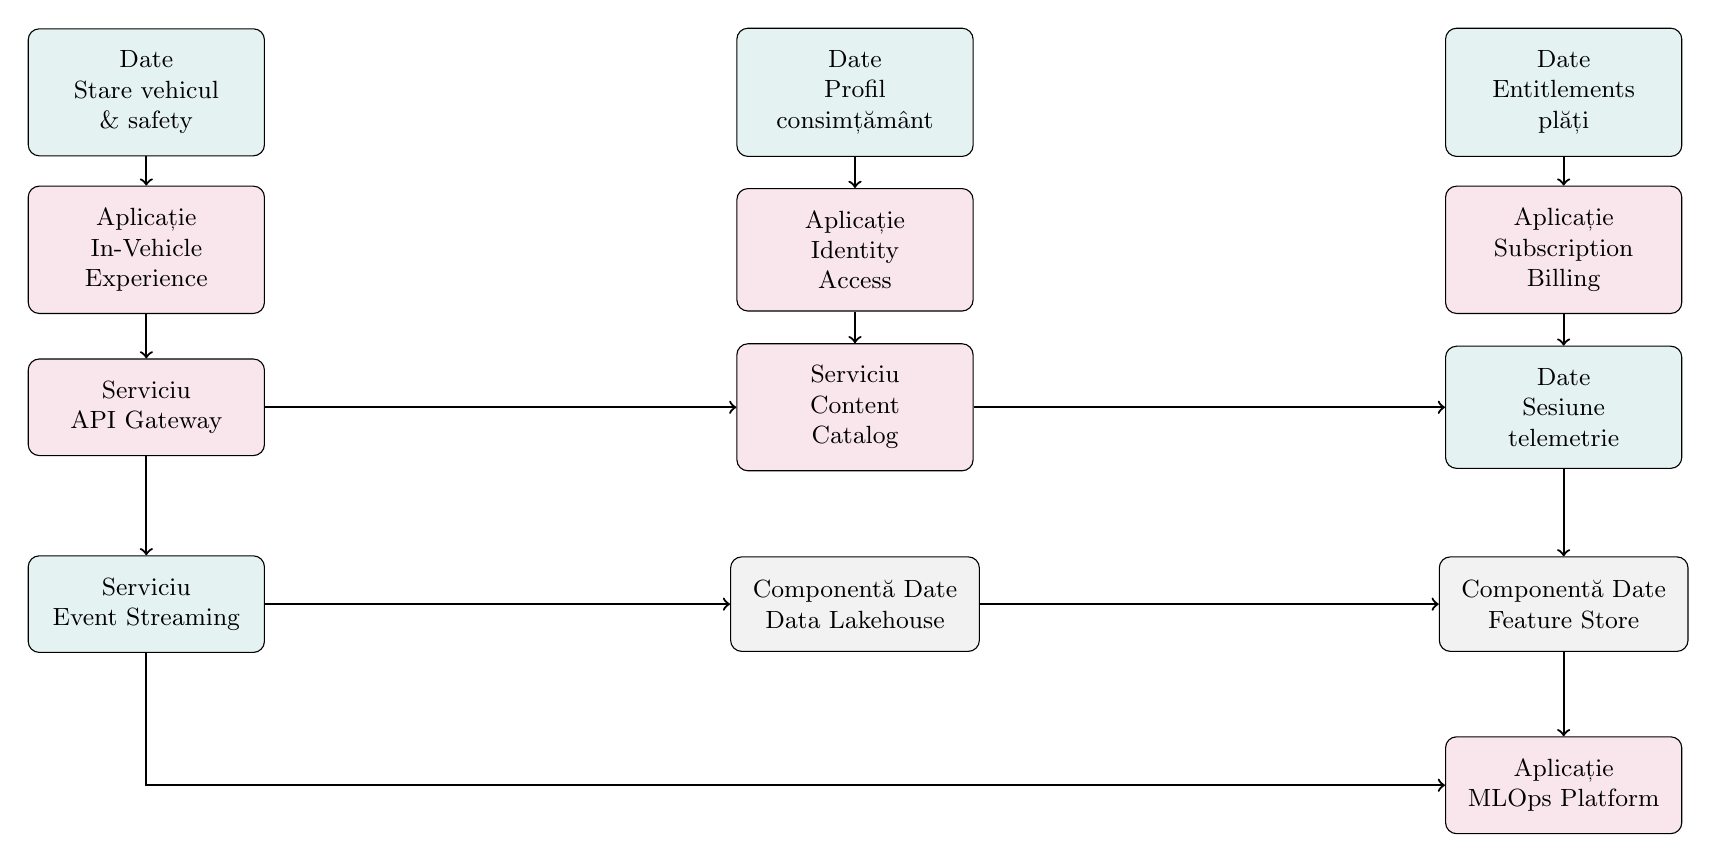
\begin{tikzpicture}[
  x=1cm,
  y=1cm,
  font=\small,
  node distance=15mm,
  box/.style={draw, rounded corners, align=center, inner sep=8pt, minimum width=3cm, minimum height=1.2cm},
  app/.style={box, fill=purple!10},
  data/.style={box, fill=teal!10},
  store/.style={box, fill=gray!10},
  arr/.style={->, thick}
]

% Layout pe grilă (3 coloane principale) cu distanțe mărite
% Coloane: Vehicle (stânga), Core Services (centru), Monetizare/AI (dreapta)

% Date (sus) - distanță orizontală mult mărită de la 7.5 la 9
\node[data] (vehState) at (-9, 4.0) {Date\\Stare vehicul\\\& safety};
\node[data] (profile)  at ( 0, 4.0) {Date\\Profil\\consimțământ};
\node[data] (ent)      at ( 9, 4.0) {Date\\Entitlements\\plăți};

% Aplicații/servicii (mijloc) - aliniate cu boxurile de sus
\node[app] (veh)     at (-9, 2.0) {Aplicație\\In-Vehicle\\Experience};
\node[app] (iam)     at ( 0, 2.0) {Aplicație\\Identity\\Access};
\node[app] (bill)    at ( 9, 2.0) {Aplicație\\Subscription\\Billing};
\node[app] (gateway) at (-9, 0.0) {Serviciu\\API Gateway};
\node[app] (content) at ( 0, 0.0) {Serviciu\\Content\\Catalog};
\node[data] (session) at ( 9, 0.0) {Date\\Sesiune\\telemetrie};

% Infrastructură/analitic (jos)
\node[data]  (stream)   at (-9,-2.5) {Serviciu\\Event Streaming};
\node[store] (lake)     at ( 0,-2.5) {Componentă Date\\Data Lakehouse};
\node[store] (features) at ( 9,-2.5) {Componentă Date\\Feature Store};
\node[app]   (mlops)    at ( 9,-4.8) {Aplicație\\MLOps Platform};

% Relații: date -> aplicații
\draw[arr] (vehState) -- (veh);
\draw[arr] (profile) -- (iam);
\draw[arr] (ent) -- (bill);

% Flux operațional (coloane verticale)
\draw[arr] (veh) -- (gateway);
\draw[arr] (gateway) -- (stream);
\draw[arr] (iam) -- (content);
\draw[arr] (bill) -- (session);

% Legătură operațională (ca în screenshot)
\draw[arr] (gateway) -- (content);
\draw[arr] (content) -- (session);

% Consolidare analitică
\draw[arr] (stream) -- (lake);
\draw[arr] (lake) -- (features);
\draw[arr] (session) -- (features);

% AI/MLOps
\draw[arr] (features) -- (mlops);
\draw[arr] (stream) |- (mlops);

\end{tikzpicture}
\end{adjustbox}
\caption{Date: diagramă de diseminare a datelor (surse, consumatori și consolidare analitică)}
\end{figure}

\subsection{Diagrama de mai jos: cooperarea aplicațiilor (Application Cooperation)}
Diagrama de cooperare a aplicațiilor oferă o imagine de ansamblu a dependențelor și interacțiunilor între aplicațiile principale. În această vizualizare, \textbf{API Gateway} are rol de integrare și expune un punct unificat pentru aplicația din vehicul, în timp ce \textbf{Identity \& Access} și \textbf{Subscription \& Billing} furnizează funcții de bază (autentificare și entitlements) necesare pentru acces la conținut.

În același timp, \textbf{Event Streaming} și \textbf{Data Lakehouse} susțin fluxul de date operaționale și analitice: telemetria produsă de vehicul este colectată și consolidată, iar \textbf{MLOps Platform} poate livra modele înapoi către runtime-ul din vehicul (ex.: detectarea anomaliilor, recomandări, îmbunătățirea safety loop). Această cooperare reflectă trecerea de la integrare „punct la punct” la o integrare controlată și scalabilă.

\begin{figure}[H]
\centering
\begin{adjustbox}{max width=\textwidth}
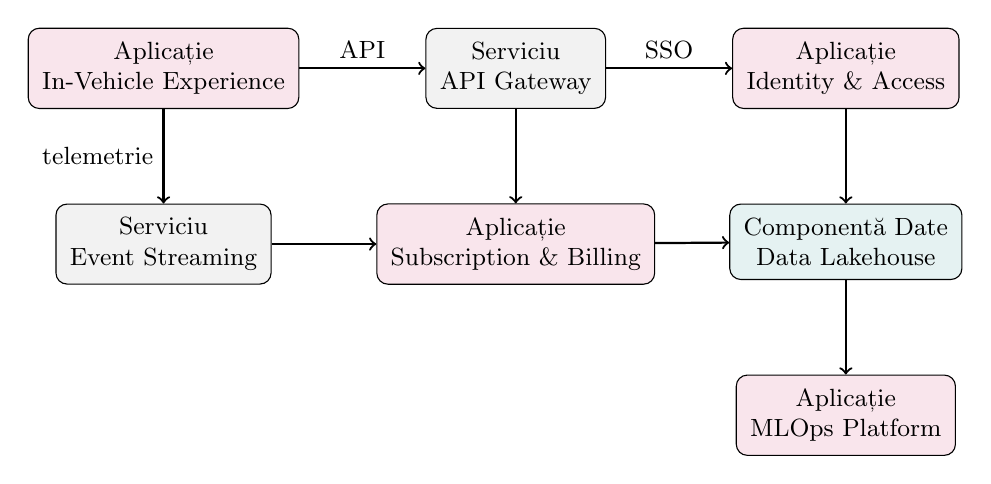
\begin{tikzpicture}[
  font=\small,
  node distance=9mm,
  box/.style={draw, rounded corners, align=center, inner sep=5pt},
  app/.style={box, fill=purple!10},
  data/.style={box, fill=teal!10},
  svc/.style={box, fill=gray!10},
  arr/.style={->, thick}
]

% Rândul superior
\node[app] (veh) {Aplicație\\In-Vehicle Experience};
\node[svc, right=16mm of veh] (api) {Serviciu\\API Gateway};
\node[app, right=16mm of api] (id) {Aplicație\\Identity \& Access};

% Rândul mijlociu
\node[svc, below=12mm of veh] (stream) {Serviciu\\Event Streaming};
\node[app, below=12mm of api] (sub) {Aplicație\\Subscription \& Billing};
\node[data, below=12mm of id] (lake) {Componentă Date\\Data Lakehouse};

% Rândul inferior
\node[app, below=12mm of lake] (ml) {Aplicație\\MLOps Platform};

% Săgeți rândul superior
\draw[arr] (veh) -- node[above]{API} (api);
\draw[arr] (api) -- node[above]{SSO} (id);

% Săgeți verticale
\draw[arr] (veh) -- node[left]{telemetrie} (stream);
\draw[arr] (api) -- (sub);
\draw[arr] (id) -- (lake);

% Săgeți orizontale rândul mijlociu
\draw[arr] (stream) -- (sub);
\draw[arr] (sub) -- (lake);

% Săgeată către MLOps
\draw[arr] (lake) -- (ml);

\end{tikzpicture}
\end{adjustbox}
\caption{Aplicații și date: cooperarea aplicațiilor (stil ArchiMate - layer aplicații + date)}
\end{figure}

\section{Faza D: Arhitectura tehnologică (Technology Architecture)}
În faza D definim infrastructura tehnologică țintă care susține arhitectura aplicațiilor și a datelor. În contextul Tesla--Meta Mobility \& Immersive, această fază este critică deoarece produsul urmărește experiențe VR în vehicul (edge) integrate cu servicii cloud la scară globală, ceea ce impune cerințe ridicate privind latența, disponibilitatea, securitatea și observabilitatea.

Scopul fazei este să descrie: platforma de execuție (compute, rețea, stocare), mediile operaționale (vehicul, cloud, corporate IT), mecanismele de securitate (PKI, management chei, policy enforcement) și capabilitățile de operare (monitorizare, logging, incident response). Prin această descriere, arhitectura tehnologică devine un „contract” tehnic între echipe: ce standarde sunt obligatorii, ce servicii sunt comune și ce dependențe trebuie respectate.

Pentru cazul nostru, arhitectura tehnologică trebuie să acopere și constrângeri specifice: conectivitate intermitentă (5G/Wi-Fi), actualizări OTA, separarea strictă a domeniilor de siguranță în vehicul, precum și integrarea cu infrastructura corporate pentru identitate și audit.

\subsection{Elemente tehnologice cheie}
\begin{itemize}[leftmargin=1.2cm]
\item \textbf{Edge (vehicul)}: compute pentru inferență, storage local, securizare hardware.
\item \textbf{Cloud region(s)}: orchestrare (Kubernetes/containers), servicii managed, rețelistică.
\item \textbf{Observabilitate}: logging, metrics, tracing, SLO.
\item \textbf{Securitate}: PKI, secrets management, policy enforcement.
\end{itemize}

\subsection{Diagrama de mai jos: infrastructură (medii și locații)}
Diagrama următoare reprezintă o vizualizare tehnologică a mediilor în care rulează soluția și a dependențelor principale dintre acestea. Ea separă trei locații:
\textbf{(1)} vehiculul (edge), unde sunt colectate datele și rulează componente locale, \textbf{(2)} cloud-ul, unde rulează serviciile scalabile și stocarea/streaming-ul de date, și \textbf{(3)} corporate IT, unde sunt operate capabilități critice de securitate și guvernanță (IAM/PKI, SOC/SIEM).

În partea de vehicul, node-ul de \textbf{edge compute} reprezintă resursele de calcul care execută runtime-ul, logica de control și inferențe locale; node-ul de \textbf{senzori \& camere} este sursa de semnale necesare atât pentru siguranță, cât și pentru telemetrie. În cloud, clusterul de aplicații și stocarea de date/streaming susțin atât fluxul operațional (API, autentificare, entitlements), cât și fluxul analitic (lakehouse, feature store, AI).

Săgețile ilustrează canale tehnologice tipice: comunicație securizată (TLS/5G) între vehicul și cloud, aplicarea politicilor și identității din corporate IT către cloud și fluxuri de audit/monitorizare din SOC către serviciile cloud. Casetele punctate sugerează granițe de rețea/segmentare, utile pentru a discuta zone de încredere și controale (ex.: zero trust, separare de domenii).

\begin{figure}[H]
\centering
\begin{adjustbox}{max width=\textwidth}
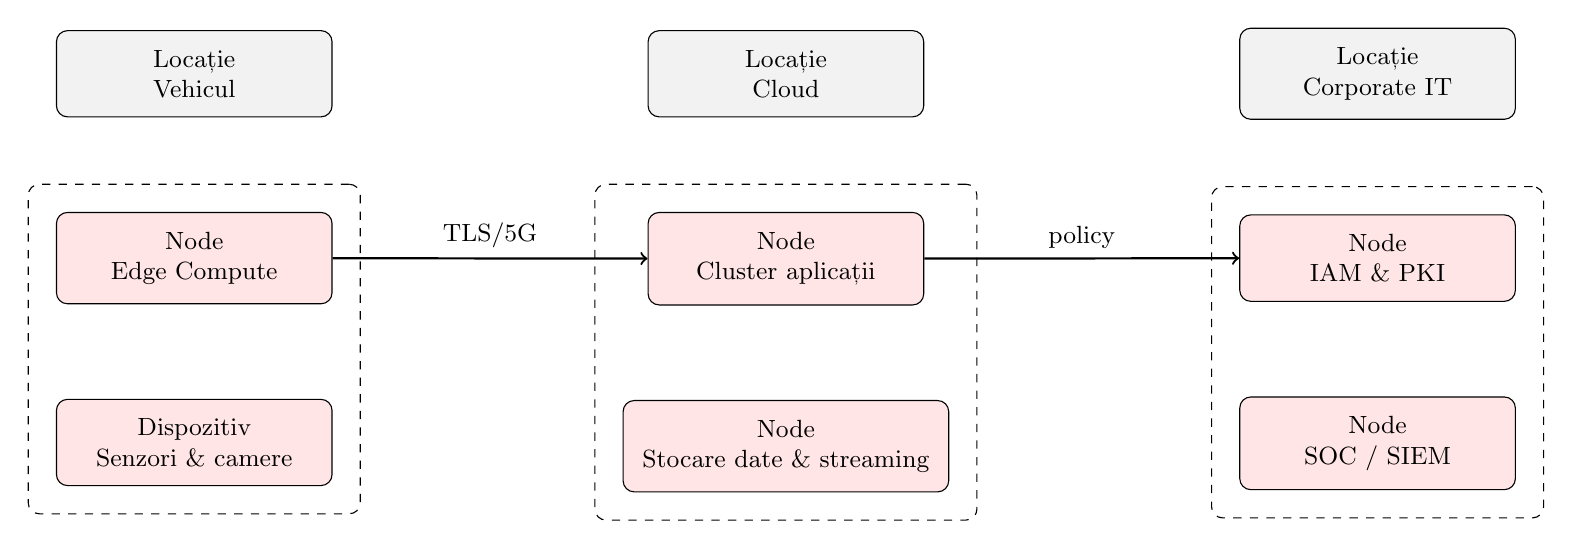
\begin{tikzpicture}[
  font=\small,
  box/.style={draw, rounded corners, align=center, inner sep=7pt, minimum width=3.5cm, minimum height=1cm},
  loc/.style={box, fill=gray!10},
  tech/.style={box, fill=red!10},
  net/.style={draw, dashed, rounded corners, inner sep=10pt},
  arr/.style={->, thick}
]

% Locații (sus) - distanță orizontală mărită
\node[loc] (car) {Locație\\Vehicul};
\node[loc, right=40mm of car] (cloud) {Locație\\Cloud};
\node[loc, right=40mm of cloud] (corp) {Locație\\Corporate IT};

% Coloane tehnologie - distanță verticală mărită
\node[tech, below=12mm of car] (edge) {Node\\Edge Compute};
\node[tech, below=12mm of edge] (sens) {Dispozitiv\\Senzori \& camere};

\node[tech, below=12mm of cloud] (k8s) {Node\\Cluster aplicații};
\node[tech, below=12mm of k8s] (data) {Node\\Stocare date \& streaming};

\node[tech, below=12mm of corp] (iam) {Node\\IAM \& PKI};
\node[tech, below=12mm of iam] (sec) {Node\\SOC / SIEM};

% Container-e cu linii punctate
\node[net, fit=(edge)(sens)] (n1) {};
\node[net, fit=(k8s)(data)] (n2) {};
\node[net, fit=(iam)(sec)] (n3) {};

% Săgeți de conexiune
\draw[arr] (edge) -- node[above]{TLS/5G} (k8s);
\draw[arr] (k8s) -- node[above]{policy} (iam);


\end{tikzpicture}
\end{adjustbox}
\caption{Tehnologie: locații și infrastructură (stil ArchiMate - layer tehnologie)}
\end{figure}

\section{Faza E: Oportunități și soluții (Opportunities \& Solutions)}
În faza E identificăm pachete de soluții și arhitecturi de tranziție care permit trecerea controlată de la baseline la arhitectura țintă. Spre deosebire de fazele C și D, care descriu sistemele și tehnologiile necesare, faza E răspunde la întrebarea cum le grupăm în inițiative implementabile, cu dependențe explicite, astfel încât să reducem riscul și să livrăm valoare incremental.

În scenariul Tesla--Meta, oportunitățile și soluțiile sunt constrânse de:
\begin{itemize}[leftmargin=1.2cm]
\item \textbf{siguranță}: funcționalități VR doar în staționare, cu controale fail-safe și auditabilitate;
\item \textbf{integrare post-fuziune}: armonizarea identității, politicilor și fluxurilor de date;
\item \textbf{scalare globală}: multi-region, latență redusă, reziliență și capacitate de operare (SRE/SOC);
\item \textbf{dependențe tehnologice}: identitate înainte de entitlement-uri, date/streaming înainte de MLOps, OTA și observabilitate ca fundație.
\end{itemize}

Rezultatul fazei este un set de pachete de lucru prioritizate, mapate pe platouri și pe arhitecturi de tranziție, astfel încât fiecare increment să poată fi guvernat și verificat prin criterii de acceptanță (security, safety, performanță, cost).

\subsection{Pachete de lucru (work packages) propuse}
\begin{itemize}[leftmargin=1.2cm]
\item \textbf{WP1 -- Identity Unification}: SSO, MFA, consimțământ și migrarea conturilor.
\item \textbf{WP2 -- Subscription \& Billing}: entitlements, facturare, integrare plăți.
\item \textbf{WP3 -- Fleet Data Platform}: ingestie telemetrie, lakehouse, catalog.
\item \textbf{WP4 -- In-Vehicle Immersive Runtime}: SDK, distribuție conținut, AR overlay.
\item \textbf{WP5 -- MLOps \& Safety Loop}: pipeline de modele, monitorizare drift, rollout controlat.
\end{itemize}

\subsection{Diagrama de mai jos: arhitecturi de tranziție (platouri) -- Figura 8}
Figura 8 reprezintă o simplificare a conceptului TOGAF de platouri: stări stabile ale arhitecturii, între care există tranziții controlate. În diagramă:
\begin{itemize}[leftmargin=1.2cm]
\item \textbf{Baseline} înseamnă sisteme separate Tesla/Meta (identitate, date și operațiuni nealiniate), cu integrare minimă și risc crescut de inconsistență.
\item \textbf{Tranziție 1} introduce fundația necesară pentru integrare: identitate unificată și primele mecanisme de guvernanță/integrare a datelor. Acest platou reduce riscul operațional și permite lansări incrementale.
\item \textbf{Target} reprezintă platforma complet integrată (edge + cloud + date + MLOps), în care funcționalitățile VR sunt livrate cu politici de siguranță și observabilitate end-to-end.
\end{itemize}

Cutii de tip work package (WP1, WP3, WP4 etc.) sunt inițiative implementabile care contribuie la atingerea unui platou. Săgețile arată relația de realizare: de exemplu, WP1 (unificarea identității) este o dependență majoră pentru acces controlat la conținut și pentru entitlements; WP3 (platforma de date) este fundația pentru observabilitate, raportare și ulterior pentru WP5 (MLOps). În final, WP4 (runtime imersiv) este livrat în forma completă atunci când fundația de identitate, date și operare este suficient de matură.

\begin{figure}[H]
\centering
\begin{adjustbox}{max width=\textwidth}
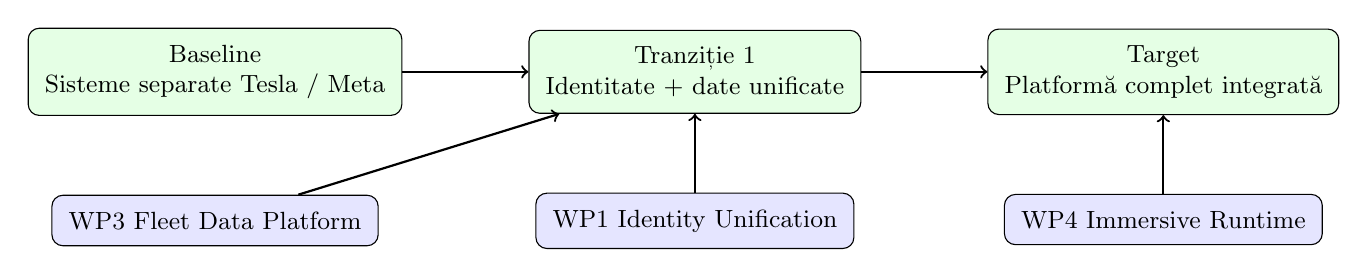
\begin{tikzpicture}[
  font=\small,
  box/.style={draw, rounded corners, align=center, inner sep=6pt},
  plateau/.style={box, fill=green!10},
  work/.style={box, fill=blue!10},
  arr/.style={->, thick}
]

\node[plateau] (p0) {Baseline\\Sisteme separate Tesla / Meta};
\node[plateau, right=16mm of p0] (p1) {Tranziție 1\\Identitate + date unificate};
\node[plateau, right=16mm of p1] (p2) {Target\\Platformă complet integrată};

\node[work, below=10mm of p1] (wp1) {WP1 Identity Unification};
\node[work, below=10mm of p2] (wp4) {WP4 Immersive Runtime};
\node[work, below=10mm of p0] (wp3) {WP3 Fleet Data Platform};

\draw[arr] (p0) -- (p1);
\draw[arr] (p1) -- (p2);
\draw[arr] (wp3) -- (p1);
\draw[arr] (wp1) -- (p1);
\draw[arr] (wp4) -- (p2);

\end{tikzpicture}
\end{adjustbox}
\caption{Migrare: platouri (baseline/tranziție/target) și pachete de lucru (stil ArchiMate - implementare 
\& migrare)}
\end{figure}

\section{Faza F: Planificarea migrației (Migration Planning)}
În faza F transformăm pachetele de lucru și arhitecturile de tranziție într-un plan de migrare realist, etapizat și guvernabil. Dacă în faza E am definit inițiativele (work packages) și către ce platou contribuie, faza F stabilește în ce ordine sunt implementate, cu ce dependențe, cu ce resurse și cu ce criterii de acceptanță.

În contextul Tesla--Meta Mobility \& Immersive, planificarea migrației trebuie să evite două riscuri majore: (1) lansarea prematură a funcționalităților VR fără fundație de siguranță și observabilitate și (2) integrarea „în cascadă” a sistemelor fără un nucleu comun de identitate, guvernanță și date. Prin urmare, roadmap-ul propus pornește cu fundațiile (identitate, observabilitate, date/streaming), continuă cu monetizarea (entitlements/billing) și finalizează cu runtime-ul imersiv și bucla MLOps.

Un rezultat important al fazei F este și definirea milestone-urilor și a criteriilor de acceptanță pentru fiecare etapă: controale de securitate (SSO/MFA, criptare, segregare acces), controale de siguranță (VR doar în staționare), indicatori de operare (SLO, latență, rata incidentelor) și criterii de migrare (compatibilitate, plan de rollback).

\subsection{Roadmap (exemplu)}
\begin{itemize}[leftmargin=1.2cm]
\item \textbf{Trimestrul 1--2}: WP1 + fundație securitate/observabilitate.
\item \textbf{Trimestrul 2--3}: WP3 (telemetrie, lakehouse, governance) + API Gateway.
\item \textbf{Trimestrul 3--4}: WP2 + primele integrări comerciale.
\item \textbf{Trimestrul 4--6}: WP4 + WP5 (MLOps) și extindere globală.
\end{itemize}

\subsection{Diagramă: timeline de migrare (Figura 9)}
\begin{figure}[H]
\centering
\begin{adjustbox}{max width=\textwidth}
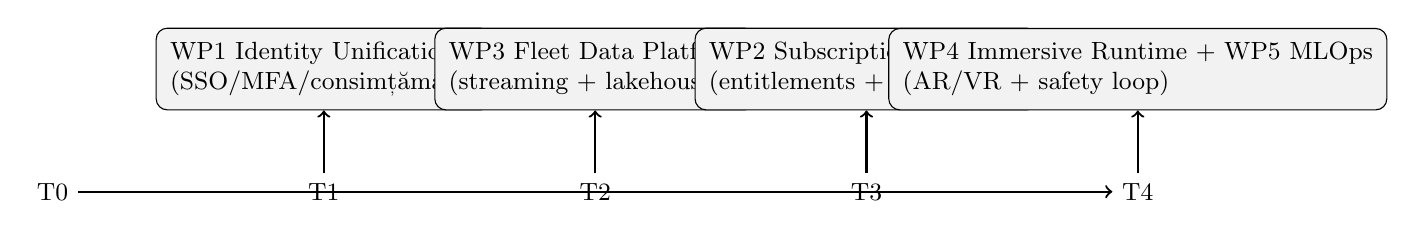
\begin{tikzpicture}[
  font=\small,
  box/.style={draw, rounded corners, align=left, inner sep=5pt, fill=gray!10},
  arr/.style={->, thick}
]

\node (t0) {T0};
\node[right=28mm of t0] (t1) {T1};
\node[right=28mm of t1] (t2) {T2};
\node[right=28mm of t2] (t3) {T3};
\node[right=28mm of t3] (t4) {T4};
\draw[arr] (t0) -- (t4);

\node[box, above=8mm of t1] (b1) {WP1 Identity Unification\\(SSO/MFA/consimțământ)};
\node[box, above=8mm of t2] (b3) {WP3 Fleet Data Platform\\(streaming + lakehouse)};
\node[box, above=8mm of t3] (b2) {WP2 Subscription \& Billing\\(entitlements + plăți)};
\node[box, above=8mm of t4] (b4) {WP4 Immersive Runtime + WP5 MLOps\\(AR/VR + safety loop)};

\draw[arr] (t1) -- (b1);
\draw[arr] (t2) -- (b3);
\draw[arr] (t3) -- (b2);
\draw[arr] (t4) -- (b4);

\end{tikzpicture}
\end{adjustbox}
\caption{Roadmap de migrare (simplificat)}
\end{figure}

\section{Faza G: Guvernarea implementării (Implementation Governance)}
Implementarea arhitecturii țintă este un proces care trebuie monitorizat și controlat, astfel încât livrările programului să rămână conforme cu arhitectura aprobată, cu cerințele de siguranță și cu cerințele de conformitate. În cazul Tesla--Meta Mobility \& Immersive, guvernanța implementării are un rol central deoarece integrarea între edge și cloud, restricția „VR doar în staționare” și cerințele de audit (GDPR, evidențe de acces, trasabilitate) impun mecanisme clare de aprobare, verificare și escaladare.

Guvernanța nu este un „checkpoint” birocratic, ci un set de reguli, responsabilități și controale care reduce riscul de derivă (implementări care se abat de la arhitectură) și crește predictibilitatea programului: ce se livrează, cine aprobă, în ce condiții se acceptă și cum se gestionează excepțiile (dispense). În faza G se operationalizează aceste aspecte prin contracte de arhitectură, evaluări de conformitate și guvernanța schimbărilor de design/implementare.

\subsection{Principii de guvernanță}
Următoarele caracteristici sunt utilizate pentru a evidenția valoarea și necesitatea guvernanței ca abordare:
\begin{itemize}[leftmargin=1.2cm]
\item \textbf{Disciplina}: echipele aderă la proceduri, procese și structuri de autoritate (Architecture Board, change control, release gates) și utilizează aceleași standarde de platformă.
\item \textbf{Transparență}: acțiunile implementate, deciziile și justificările (inclusiv dispense) sunt înregistrate și accesibile pentru audit intern și extern.
\item \textbf{Independență}: mecanismele de verificare (security review, safety review, evaluare de conformitate) sunt organizate astfel încât să minimizeze conflictele de interese.
\item \textbf{Responsabilitate}: grupurile care decid (CIO, Architecture Board, Security/Safety Office, SRE/SOC) sunt autorizate și răspunzătoare pentru deciziile lor.
\item \textbf{Corectitudine}: criteriile de acceptanță și procesele sunt aplicate uniform, fără a crea avantaje nedrepte pentru o anumită echipă/furnizor.
\end{itemize}

\subsection{Modelul de guvernanță (Figura 15)}

\begin{figure}[H]
\centering
\begin{adjustbox}{max width=\textwidth}
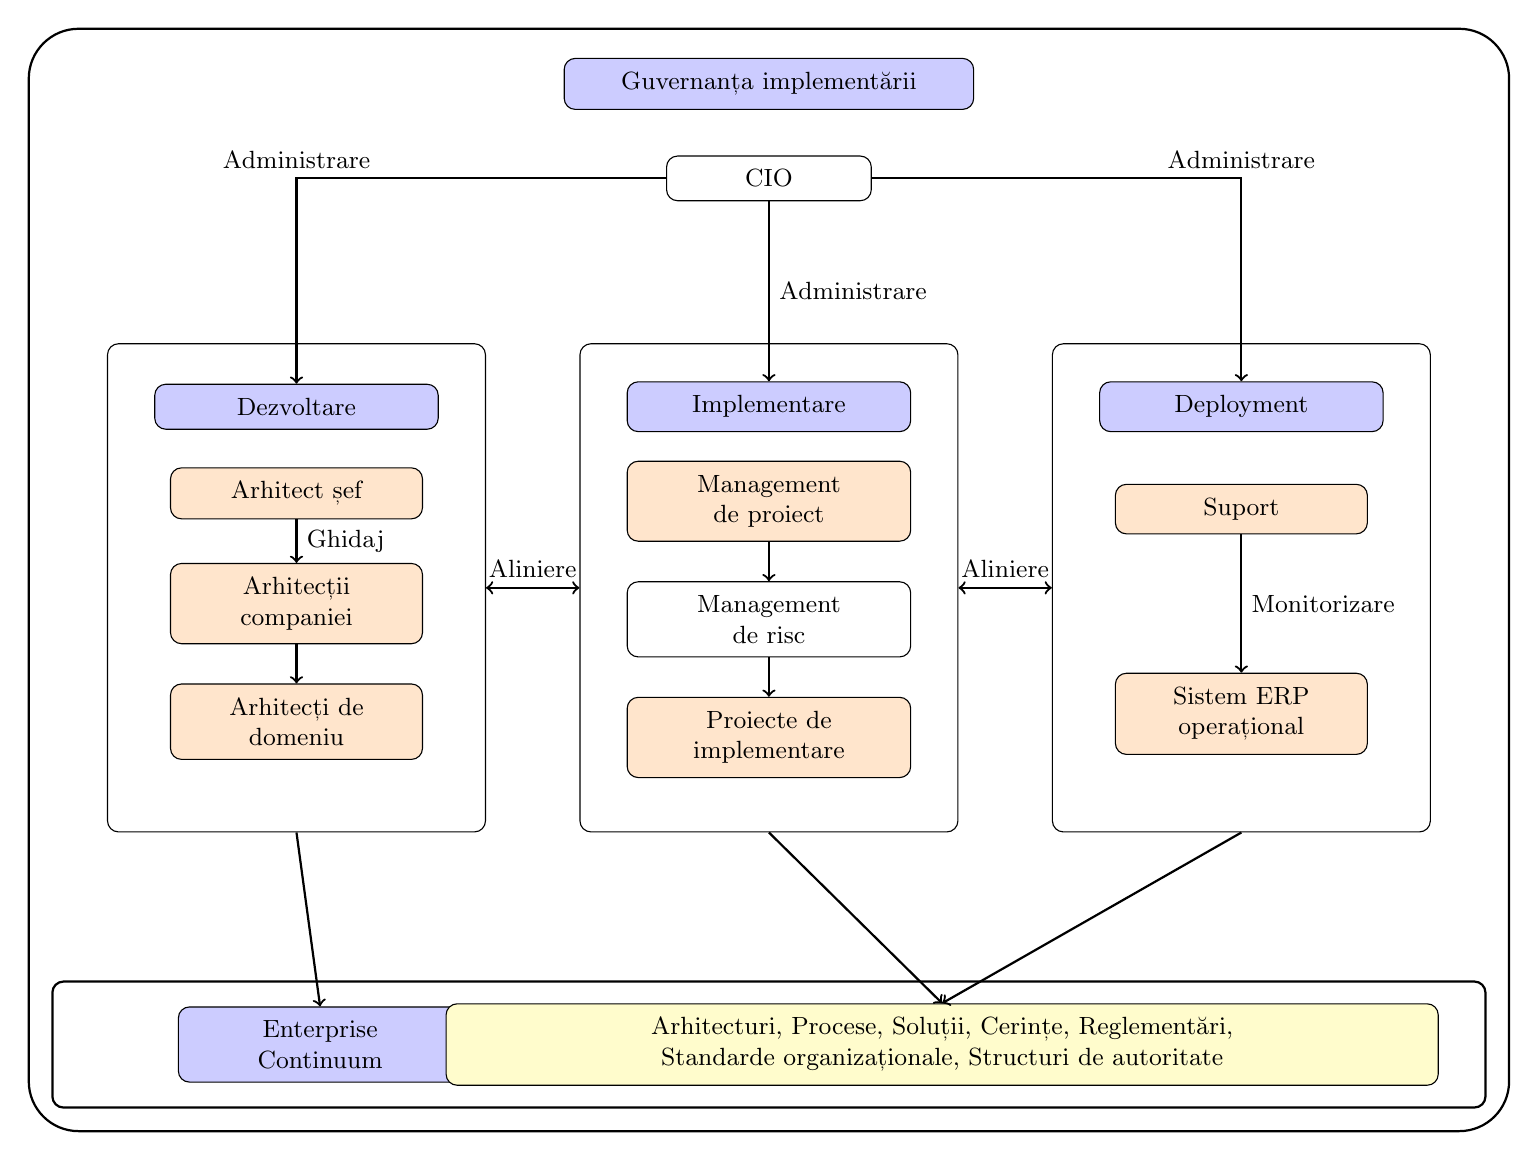
\begin{tikzpicture}[
  x=1cm,
  y=1cm,
  font=\small,
  box/.style={draw, rounded corners, align=center, inner sep=5pt},
  title/.style={box, fill=blue!20},
  role/.style={box, fill=orange!20},
  panel/.style={draw, rounded corners, minimum width=4.8cm, minimum height=6.2cm},
  arr/.style={->, thick},
  bidi/.style={<->, thick}
]

\draw[draw, rounded corners=18pt, thick] (-9.4,-8.5) rectangle (9.4,5.5);

\node[title, minimum width=5.2cm] (gov) at (0,4.8) {Guvernanța implementării};
\node[box, minimum width=2.6cm] (cio) at (0,3.6) {CIO};

\node[panel] (pDev) at (-6,-1.6) {};
\node[panel] (pImpl) at (0,-1.6) {};
\node[panel] (pDep) at (6,-1.6) {};

\node[title, minimum width=3.6cm] (dev) at (-6,0.7) {Dezvoltare};
\node[role, minimum width=3.2cm] (archChief) at (-6,-0.4) {Arhitect șef};
\node[role, minimum width=3.2cm] (archCo) at (-6,-1.8) {Arhitecții\\companiei};
\node[role, minimum width=3.2cm] (archDom) at (-6,-3.3) {Arhitecți de\\domeniu};

\node[title, minimum width=3.6cm] (impl) at (0,0.7) {Implementare};
\node[role, minimum width=3.6cm] (pm) at (0,-0.5) {Management\\de proiect};
\node[box, minimum width=3.6cm] (rm) at (0,-2.0) {Management\\de risc};
\node[role, minimum width=3.6cm] (proj) at (0,-3.5) {Proiecte de\\implementare};

\node[title, minimum width=3.6cm] (dep) at (6,0.7) {Deployment};
\node[role, minimum width=3.2cm] (support) at (6,-0.6) {Suport};
\node[role, minimum width=3.2cm] (ops) at (6,-3.2) {Sistem ERP\\operațional};

\draw[arr] (cio) -| node[above]{Administrare} (dev.north);
\draw[arr] (cio) -- node[right]{Administrare} (impl.north);
\draw[arr] (cio) -| node[above]{Administrare} (dep.north);

\draw[arr] (archChief) -- node[right]{Ghidaj} (archCo);
\draw[arr] (archCo) -- (archDom);

\draw[arr] (pm) -- (rm);
\draw[arr] (rm) -- (proj);

\draw[arr] (support) -- node[right]{Monitorizare} (ops);

\draw[bidi] (pDev.east) -- node[above]{Aliniere} (pImpl.west);
\draw[bidi] (pImpl.east) -- node[above]{Aliniere} (pDep.west);

% Dreptunghi care cuprinde Enterprise Continuum și caseta cu standarde
\draw[draw, rounded corners, thick] (-9.1,-8.2) rectangle (9.1,-6.6);

\node[title, minimum width=3.6cm] (ec) at (-5.7,-7.4) {Enterprise\\Continuum};
\node[box, fill=yellow!20, minimum width=12.6cm] (std) at (2.2,-7.4) {Arhitecturi, Procese, Soluții, Cerințe, Reglementări,\\Standarde organizaționale, Structuri de autoritate};

\draw[arr] (pDev.south) -- (ec.north);
\draw[arr] (pImpl.south) -- (std.north);
\draw[arr] (pDep.south) -- (std.north);

\end{tikzpicture}
\end{adjustbox}
\caption{Figura 15: Modelul de guvernanță}
\end{figure}

\subsection{Reguli și procedee de guvernanță}
Pentru a asigura o abordare consecventă, compania urmează o serie de reguli și procedee de guvernanță:
\begin{enumerate}[leftmargin=1.2cm]
\item Crearea de bune practici pentru transmiterea, adoptarea, reutilizarea, raportarea și retragerea politicilor de arhitectură, procedurilor, rolurilor, competențelor, structurilor organizaționale și serviciilor de asistență.
\item Responsabilități și structuri organizaționale care sprijină procesele de guvernanță a arhitecturii și cerințele de raportare.
\item Integrarea instrumentelor și proceselor pentru a facilita preluarea proceselor, atât din punct de vedere procedural, cât și cultural.
\item Criterii pentru control: dispense, evaluări de conformitate, revizii periodice și criterii de acceptanță pentru release.
\item Cerințe interne și externe privind eficacitatea, eficiența, confidențialitatea, integritatea, disponibilitatea, conformitatea și fiabilitatea informațiilor, serviciilor și proceselor.
\end{enumerate}

\subsection{Contract de arhitectură (elemente)}
\begin{itemize}[leftmargin=1.2cm]
\item scope-ul pachetelor de lucru și criteriile de acceptanță;
\item standarde obligatorii (identitate, logging, criptare, API versioning) și controale de siguranță (VR doar în staționare);
\item măsurători: SLO, cost per user, latență, rata incidentelor;
\item proces de conformitate (review-uri de arhitectură, security review, threat modeling) și gestionarea excepțiilor (dispense).
\end{itemize}

\section{Faza H: Managementul schimbărilor arhitecturale (Architecture Change Management)}
Faza H menține arhitectura relevantă și controlată după ce inițiativele au intrat în operare. În loc să tratăm arhitectura ca un document „final”, faza H instituie un mecanism de schimbare continuă: colectăm semnale (triggeri), formulăm cereri de schimbare, evaluăm impactul asupra arhitecturilor (Business/Data/Application/Technology) și actualizăm standardele, principiile și roadmap-ul.

Pentru Tesla--Meta Mobility \& Immersive, această fază are o importanță suplimentară deoarece produsul este expus unor schimbări rapide: evoluții legislative (GDPR, AI Act), amenințări de securitate, schimbări de platformă (device-uri AR/VR, SDK-uri), precum și lecții din exploatare (incidente, degradări de performanță, drift de modele). Faza H asigură că aceste schimbări nu duc la „derivă” arhitecturală și că deciziile rămân trasabile.


\subsection{Evaluarea impactului și decizia}
Pentru fiecare schimbare relevantă se evaluează impactul asupra:
\begin{itemize}[leftmargin=1.2cm]
\item \textbf{arhitecturii de date}: fluxuri de date, retenție, consimțământ, calitate, catalog;
\item \textbf{arhitecturii aplicațiilor}: contracte API, integrare, compatibilitate, versionare;
\item \textbf{arhitecturii tehnologice}: topologie, politici de securitate, observabilitate, cost și scalare;
\item \textbf{operării}: SLO/SLI, runbook-uri, on-call, rollback și change management.
\end{itemize}
Decizia se ia în forul de guvernanță potrivit (Architecture Board / Security \& Safety / CAB), iar rezultatul este fie aprobare, fie respingere, fie aprobare condiționată (cu acțiuni corective și criterii de acceptanță).

\subsection{Actualizarea arhitecturii și a artefactelor}
O schimbare aprobată trebuie reflectată în mod controlat în documentație și în practicile curente:
\begin{itemize}[leftmargin=1.2cm]
\item actualizarea principiilor, standardelor și „best practices” (inclusiv policy-as-code acolo unde e posibil);
\item actualizarea diagramelor și a contractelor de arhitectură;
\item actualizarea roadmap-ului și a platourilor (dacă schimbarea este majoră);
\item comunicare către echipe și includerea în release planning (cu verificări de conformitate).
\end{itemize}

\section{Concluzii finale}
Aplicarea TOGAF ADM pentru proiectul „Fuziune Tesla--Meta” a permis parcurgerea etapelor de la definirea contextului și a viziunii până la guvernanță și schimbare continuă, obținând o arhitectură coerentă, guvernabilă și livrabilă incremental.

În fazele inițiale au fost clarificate scopul și cerințele, părțile interesate și obiectivele, apoi a fost modelată arhitectura de business și au fost stabilite principiile care ghidează deciziile. Ulterior, au fost definite arhitecturile de date și aplicații (fluxuri, integrare și dependențe) și arhitectura tehnologică necesară pentru execuția edge--cloud, securitate și observabilitate.

În fazele de planificare și execuție, soluțiile au fost organizate în work packages și platouri, apoi transformate într-un roadmap de migrare cu dependențe și criterii de acceptanță. În final, guvernanța implementării și managementul schimbării arhitecturale au stabilit mecanisme de control, conformitate și actualizare a artefactelor, astfel încât platforma Tesla--Meta VR (cu constrângerea „VR doar în staționare”) să poată evolua controlat, respectând cerințe de siguranță, securitate și GDPR.

\section{test}